\chapter{Формула Пуассона решения задачи Коши для волнового уравнения в $R^2$. Метод спуска.}
\label{cha:8}

Имеем задачу Коши для волнового уравнения в $\mathbb{R}^2$:
$$\begin{cases}
	u_{tt} = a^2 \triangle_{\overline{x}} u, \; t > 0, \; \overline{x} \in \mathbb{R}^2 \\
	\left.
  		\begin{array}{ccc}
    		u|_{t=0} = \varphi(x) \\
    		u_t |_{t=0} = \psi (x)
  		\end{array}
	\right\}, \; \overline{x} \in \mathbb{R}^2
\end{cases}$$
\begin{theorem}[\red{формула Пуассона}]\label{lec:8/the:1}
	Формула решения задачи Коши для волнового уравнения в $\mathbb{R}^2$ имеет вид:
	$$u(t, \overline{x}) = \frac{1}{2 \pi a} \underset{|\overline{x} - \xi| \leq at}{\overset{}{\iint}} \dfrac{\psi (\overline{\xi}) d \bar{\xi} }{\sqrt{(at)^2 - |\bar{\xi} - \bar{x}|^2}} + \frac{\partial}{\partial t} (\frac{1}{2 \pi a} \underset{|\overline{x} - \xi| \leq at}{\overset{}{\iint}} \dfrac{\varphi (\overline{\xi}) d \bar{\xi} }{\sqrt{(at)^2 - |\bar{\xi} - \bar{x}|^2}}) $$
\end{theorem}
\begin{Proof}
Пусть $u (t, x_1, x_2, x_3)$ - решение задачи Коши в $\mathbb{R}^3$:
$$\begin{cases}
	u_{tt} = a^2 \triangle_{\overline{x}} u, \; t > 0, \; \overline{x} \in \mathbb{R}^3 \\
	\left.
  		\begin{array}{ccc}
    		u|_{t=0} = \varphi(x_1, x_2) \\
    		u_t |_{t=0} = \psi (x_1, x_2)
  		\end{array}
	\right\}, \; \overline{x} \in \mathbb{R}^3
\end{cases}\eqno(*)$$
Пространство трехмерное, но начальные условия зависят только от $x_1, x_2$. Решение такой задачи находится по формуле Кирхгофа.\\
Сделае сдвиг по оси $x_3$ на $x_3^0 \in \mathbb{R}$. Функция $u(t,x)$ перейдет в $\tilde{u}(t, \overline{x}) = u (t, x_1, x_2, x_3+x_3^0)$. Но волновое уравнение от сдвига по оси не изменится, как не изменятся и начальные условия. Тогда $\tilde{u}(t,\overline{x})$ является решением задачи $(*)$, как и функция $u(t,\overline{x})$. В силу единственности решения задачи Коши $(*)$ $\tilde{u}(t,\overline{x}) = u(t,\overline{x})$, т.е. $u(t, \overline{x})$ не зависит от $x_3$.\\

Вернемся к исходной двумерной задаче: $u = u (t, x_1, x_2)$. Тогда $\frac{\partial^2 u}{\partial x_3^2} = 0$, значит $u(t, \overline{x})$, задаваемая формулой Кирхгофа, является и решением двумерной задачи Коши, если начальные условия не зависят от $x_3$.\\

Разобьем исходную задаче на две:
$$\begin{gathered}
		u = u_1 + u_2 \\
	\begin{cases}
		(u_1)_{tt} = a^2 \triangle_{\overline{x}} u_1 \\
		(u_1)|_{t = 0} = \varphi (x_1, x_2) \\
		(u_1)_t |_{t = 0} = 0
	\end{cases}
	\begin{cases}
		(u_2)_{tt} = a^2 \triangle_{\overline{x}} u_2 \\
		(u_2)|_{t = 0} = 0 \\
		(u_2)_t |_{t = 0} = \psi (x_1, x_2)
	\end{cases}
\end{gathered}$$
По формуле Кирхгофа получаем:
$$u_2 (t, x_1, x_2) = \frac{1}{4\pi a^2 t} \underset{|\overline{\xi}-\overline{x}|=at}{\overset{}{\varoiint}}\psi (\xi_1, \xi_2)d \sigma_{\xi}$$
Сведем интегрирование по сфере к интегрированию в $\mathbb{R}^2$:

\begin{figure}[h]
	\begin{multicols}{2}
		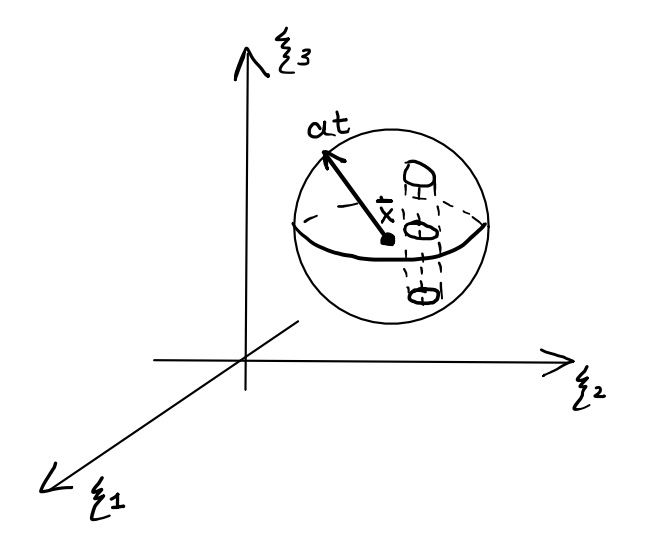
\includegraphics[width=80mm]{cha8im1}
		\columnbreak
		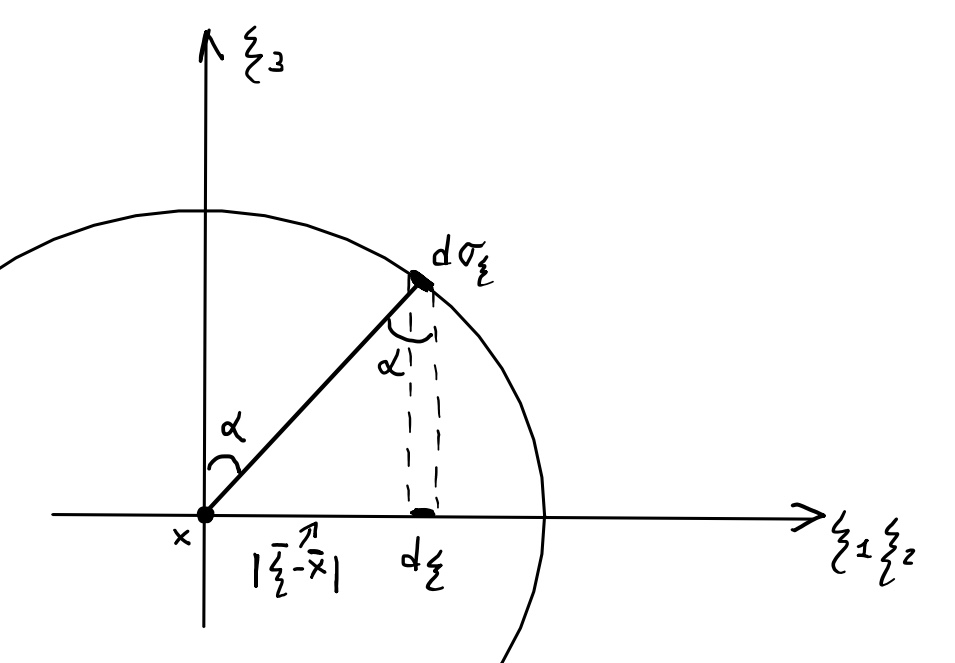
\includegraphics[width=90mm]{cha8im2}
	\end{multicols}
\end{figure}
Сфера проектируется на круг $|\overline{\xi}-\overline{x}|\le at$, $\alpha$ - угол между нормалью к сфере и $\xi_3$, $d \sigma_{\xi}$ - элемент площади на сфере, $d\xi = d\xi_1 d\xi_2$ - элемент площади на круге.
$$\sin{\alpha} = \frac{|\overline{\xi}-\overline{x}|}{a t} \; \Rightarrow \; \cos{\alpha} = \sqrt{1 - \frac{|\overline{\xi}-\overline{x}|^2}{a^2 t^2}} = \frac{\sqrt{a^2t^2|\overline{\xi}-\overline{x}|^2}}{a t} = \frac{d\xi}{d \sigma_{\xi}}$$
Отсюда получаем:
$$u_2 (t, x_1, x_2) = \frac{2}{4\pi a^2 t} \underset{|\overline{\xi}-\overline{x}|\le at}{\overset{}{\iint}}\psi (\xi_1, \xi_2) \frac{d\xi \cdot at}{\sqrt{a^2t^2 - |\overline{\xi}-\overline{x}|^2}} = \frac{1}{2\pi a}\underset{|\overline{\xi}-\overline{x}|\le at}{\overset{}{\iint}} \frac{\psi (\xi_1, \xi_2) d\xi_1 d\xi_2}{\sqrt{a^2t^2 - |\overline{\xi}-\overline{x}|^2}}$$
Умножение на $2$ происходит, потому что в каждую точку круга проецируется две точки сферы (с верхней и нижней частей). Итак, формула Пуассона имеет вид (аналогично формуле Кирхгофа):
$$u(t, \overline{x}) = \frac{1}{2 \pi a} \underset{|\overline{x} - \xi| \leq at}{\overset{}{\iint}} \dfrac{\psi (\overline{\xi}) d \bar{\xi} }{\sqrt{(at)^2 - |\bar{\xi} - \bar{x}|^2}} + \frac{\partial}{\partial t} (\frac{1}{2 \pi a} \underset{|\overline{x} - \xi| \leq at}{\overset{}{\iint}} \dfrac{\varphi (\overline{\xi}) d \bar{\xi} }{\sqrt{(at)^2 - |\bar{\xi} - \bar{x}|^2}}) $$















% Делаем все то же самое, что для формулы Кирхгофа:

% $$\begin{cases}
% 	u_{tt} = a^2 \triangle_{\overline{x}} u, \; t > 0, \; x \in \mathbb{R}^3 \\
% 	u|_{t = 0} = 0 \\
% 	u_t |_{t = 0} = \psi (x_1, x_2)
% \end{cases}$$

% $$
% u(t,x) = \dfrac{1}{2}\underset{|\overline{x} - \xi| \leq at}{\overset{}{\iint}}\dfrac{\psi (\overline{\xi}) d \sigma_\xi }{\sqrt{(at)^2 - |\bar{\xi} - \bar{x}|^2}} 
% $$

% Запишем решение с помощью формулы Кирхгофа для трехмерного случая, считая, что $ \psi = \psi(x_1, x_2): $

% $$
% u(t,x) = \frac{1}{4 \pi a^2 t} \underset{|\overline{x} - \xi| = at}{\overset{}{\varoiint}} \psi (\xi_1, \xi_2) d \sigma_\xi.
% $$

% \begin{center}
% 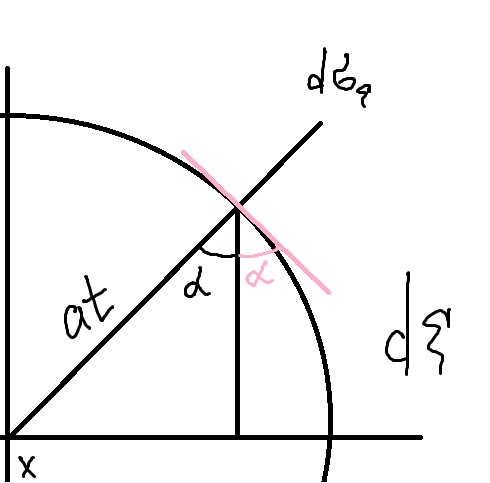
\includegraphics[scale=0.6]{dsigma}
% \end{center}

% $$
% \begin{gathered}
% d\sigma_{\xi} = \dfrac{d\xi}{\cos(\alpha)}, \\
% \sin(\alpha) = \dfrac{|\xi - x|}{at} \longrightarrow \cos(\alpha) = \sqrt{1 - \dfrac{|\xi - x|^2}{(at)^2}} = \dfrac{\sqrt{(at)^2 - |\xi - x|^2}}{at},
% \end{gathered}
% $$

% тогда 

% $$
% u(t, \overline{x}) = \frac{2at}{4 \pi a^2 t} \underset{|\overline{x} - \xi| \leq at}{\overset{}{\iint}} \dfrac{\psi (\overline{\xi}) d \bar{\xi} }{\sqrt{(at)^2 - |\bar{\xi} - \bar{x}|^2}} = \frac{1}{2 \pi a} \underset{|\overline{x} - \xi| \leq at}{\overset{}{\iint}} \dfrac{\psi (\overline{\xi}) d \bar{\xi} }{\sqrt{(at)^2 - |\bar{\xi} - \bar{x}|^2}}
% $$

% В числителе появилась 2, так как в каждую очку круга проецируются две очки сферы (с верхней и нижней частей). Итак, \red{формула Пуассона}:

% $$u(t, \overline{x}) = \frac{1}{2 \pi a} \underset{|\overline{x} - \xi| \leq at}{\overset{}{\iint}} \dfrac{\psi (\overline{\xi}) d \xi_1\xi_2 }{\sqrt{(at)^2 - |\bar{\xi} - \bar{x}|^2}} + \frac{\partial}{\partial t} (\frac{1}{2 \pi a} \underset{|\overline{x} - \xi| \leq at}{\overset{}{\iint}} \dfrac{\varphi (\overline{\xi}) d \bar{\xi} }{\sqrt{(at)^2 - |\bar{\xi} - \bar{x}|^2}}) $$
\end{Proof}

Метод, позволяющий свести задачу большей размерности к задаче меньшей размерности, называется \red{методом спуска}.
